\subsection{Controller and Plant Testing}
\label{sec:pwrtesting}

\subsubsection{Plant Tests}

On creation of the plant, components needed to be tested to ensure operation were as expected.
Step responses were observed for the components (Figure \ref{fig:power-risetime}), which conformed to expectations (as in Table \ref{tbl:time}) and the test was deemed successful.

\begin{figure}[ht]
    \centering
    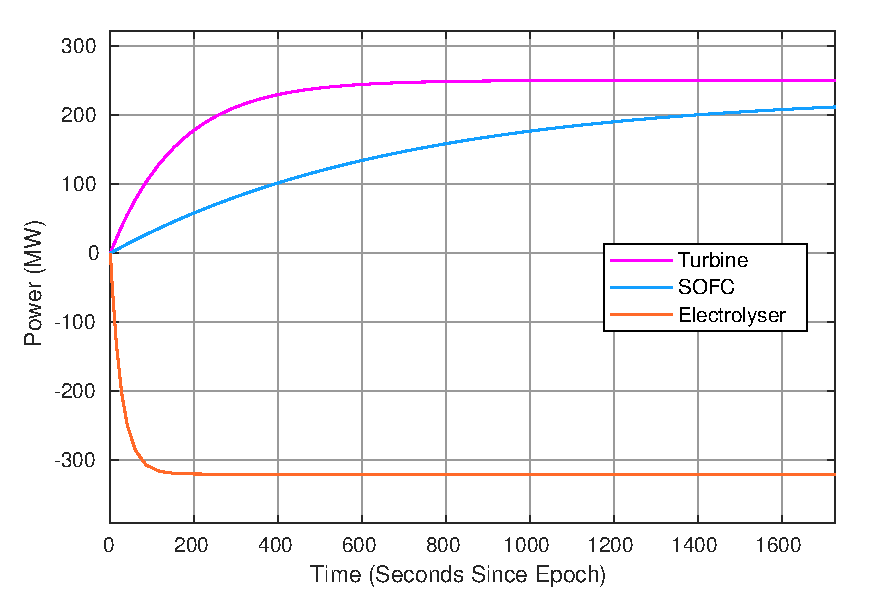
\includegraphics[scale=0.5]{images/results/risetime.eps}
    \caption{Tests conducted on Power Components with differing rise times.}
    \label{fig:power-risetime}
\end{figure}

Tanks were tested and operated as expected, parameters for the Haber-Bosch, and cryogenic still were added and the plant behaved as expected.

An important note for all the controllers that were experimented on was that the electrical inertia $J$ was reduced until the plant could no longer be controlled within tolerances, and then a small safety factor was added.
Interestingly all controllers had a similar lower limit on the tolerable inertia.
It was decided $J = 80 \cdot 10^{3}\text{kgm}^{2}$.

\subsubsection{Proportional Control}

A proportional control scheme was initially applied to observe how the system responds and check stability.
Results of the simulation are visible in Figure \ref{fig:power-proportional}.

\begin{figure}[]ht]
\centering
\begin{subfigure}{.5\textwidth}
  \centering
  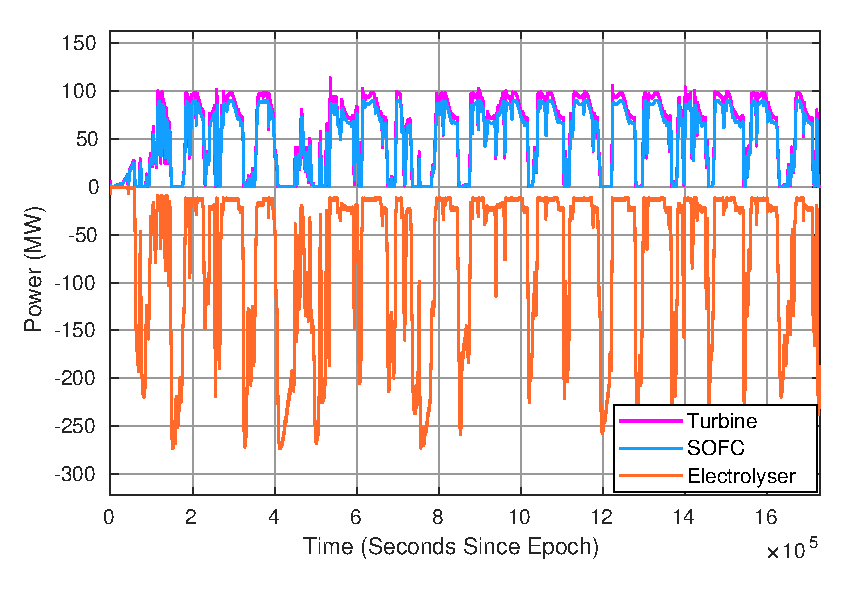
\includegraphics[width=1\linewidth]{images/results/P/use.eps}
  \caption{Component powers.}
  \label{fig:sub1}
\end{subfigure}%
\begin{subfigure}{.5\textwidth}
  \centering
  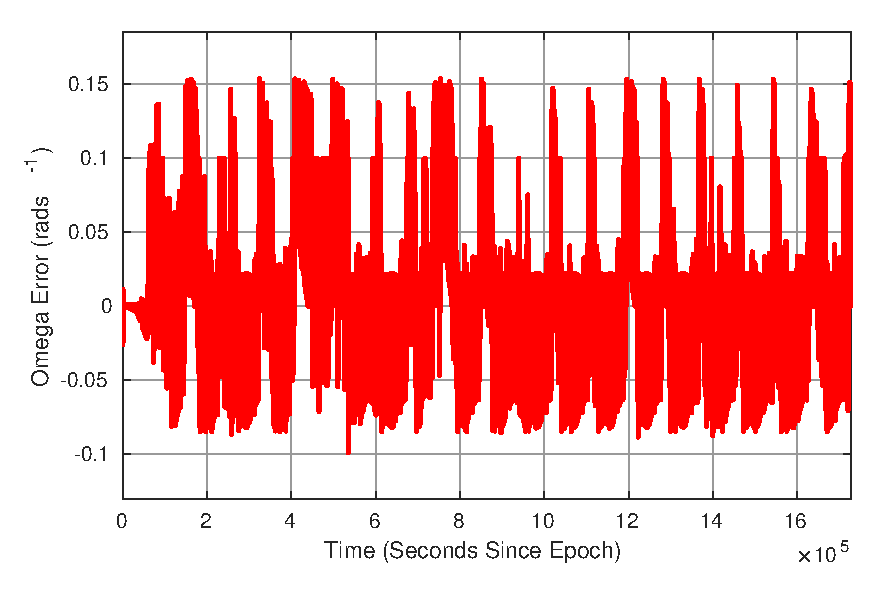
\includegraphics[width=1\linewidth]{images/results/P/omega.eps}
  \caption{Frequency error from 120 $\pi$ rads$^{-1}$.}
  \label{fig:sub2}
\end{subfigure}
\caption{Simulation results from a 100 days of data, {\bf Proportional Control Applied, $P=10$.}}
\label{fig:power-proportional}
\end{figure}

System was found to be stable, but had steady state tracking errors.
The turbine running at DC was not desirable, so a PID in parallel with a Proportional unit was applied as suggested in Section \ref{sec:power-pid}.





%%%%%% PID PART 1






\subsubsection{Plant with a PID/PD Combination}

By implementing the same method as suggested in Section \ref{sec:power-pid}, the following results were yielded.
Important to note was very strong performance from the controller, where very low frequency error is visible.
This unfortunately came at the cost of an high ammonia use-rate, ending the 100 day simulation at -4200 tons of ammonia.

\begin{figure}[ht]
\centering
\begin{subfigure}{.5\textwidth}
  \centering
  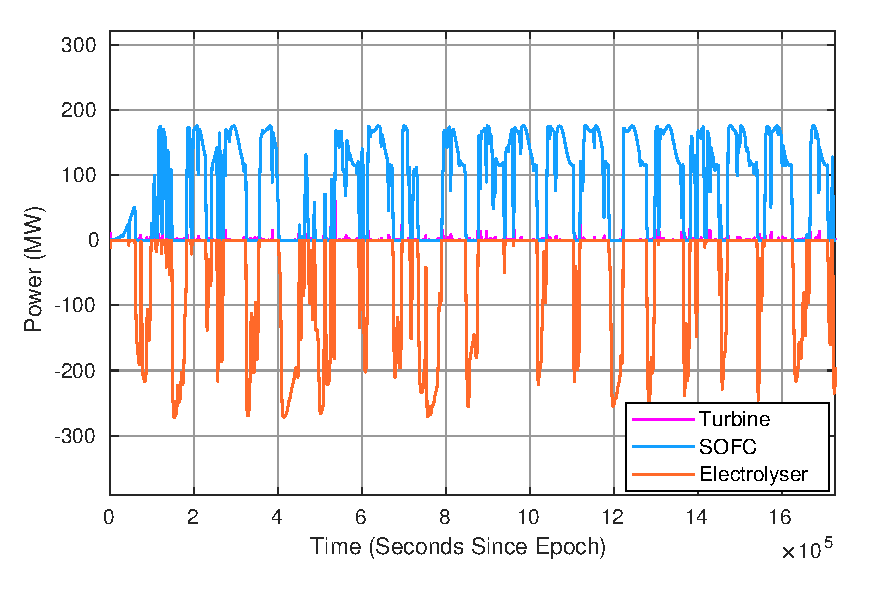
\includegraphics[width=1\linewidth]{images/results/PID/power.eps}
  \caption{Component powers.}
  \label{fig:piduse}
\end{subfigure}%
\begin{subfigure}{.5\textwidth}
  \centering
  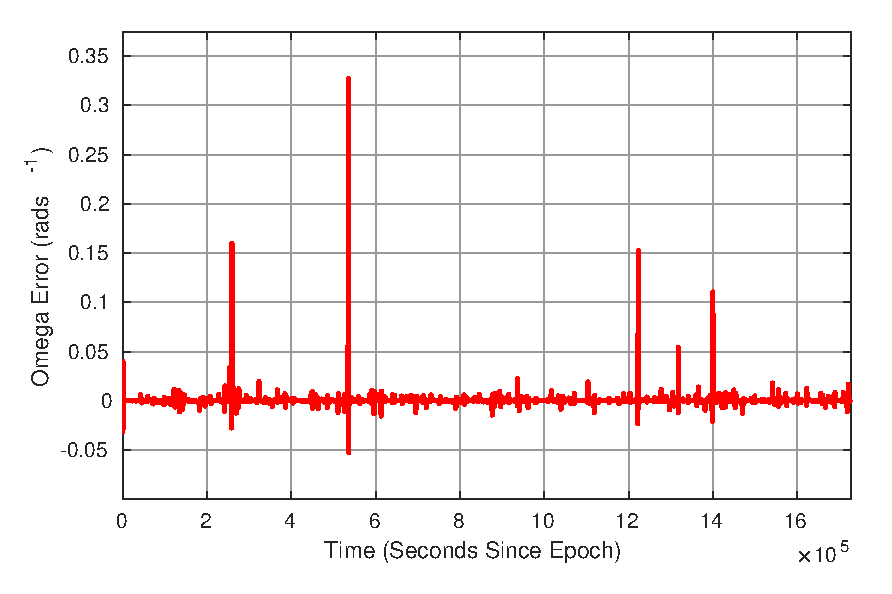
\includegraphics[width=1\linewidth]{images/results/PID/omega.eps}
  \caption{Frequency error from 120 $\pi$ rads$^{-1}$.}
  \label{fig:pidpower}
\end{subfigure}
\caption{Simulation results from a 100 days of data, {\bf PID in Parallel with Proportional Control Applied, $P= 10,I= 0.2,D= 0.8, P_{\mathrm{turbine}} = 10$.}}
\label{fig:power-PID-sim}
\end{figure}








%%%%% LQR PART 2







\subsubsection{Plant with a Augmented LQR Combination}

System was able to perform well under simulated harsh conditions, with a manageable frequency error.

Compared to PID, there is a significantly larger frequency error, however it is comfortably within tolerances.
Interestingly the LQR used less ammonia than the PID, ending the 100 day simulation with -3850 tons of ammonia.

The Augmented LQR Combination was preferred and then run for a year, to ensure the material balance and error tolerance satisfied expectations.



\begin{figure}[ht]
\centering
\begin{subfigure}{.5\textwidth}
  \centering
  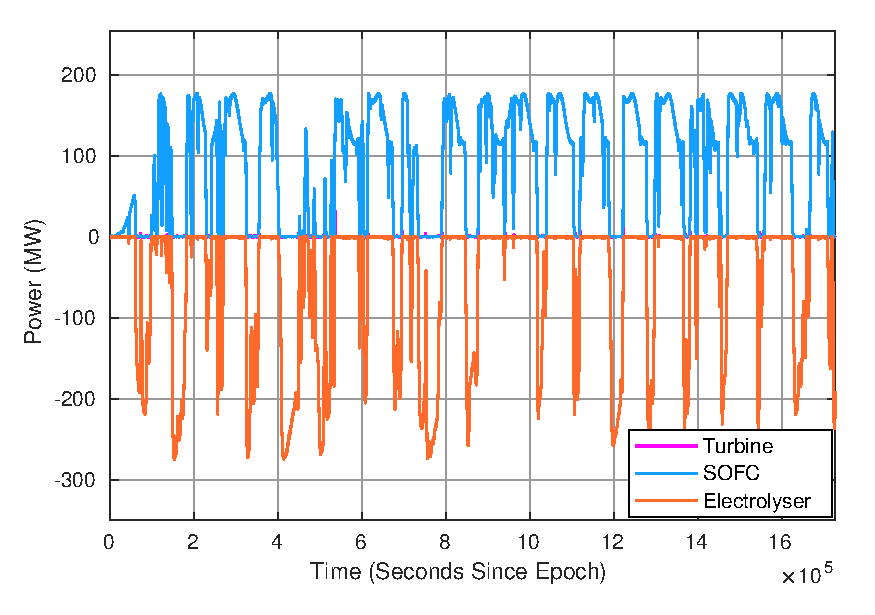
\includegraphics[width=1\linewidth]{images/results/LQR/use.eps}
  \caption{Component powers.}
  \label{fig:lqruse}
\end{subfigure}%
\begin{subfigure}{.5\textwidth}
  \centering
  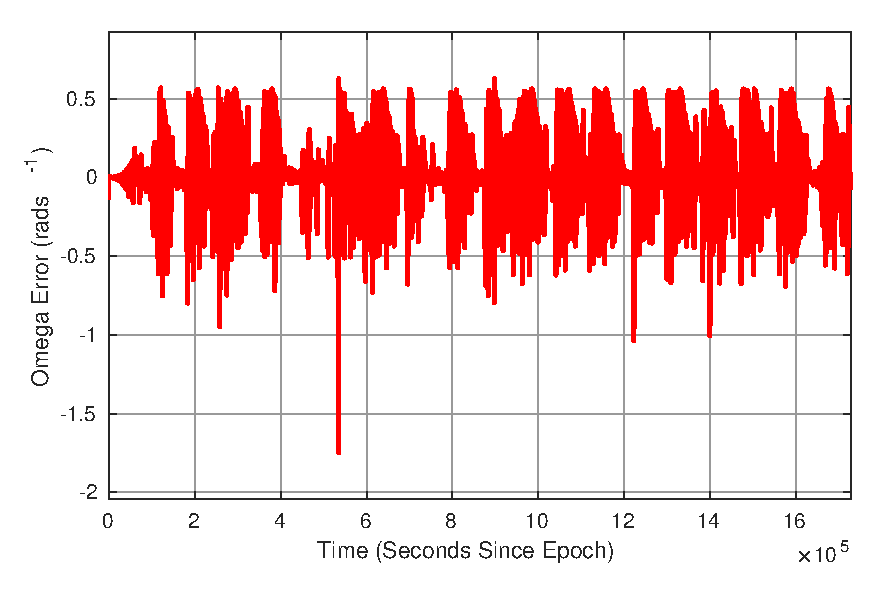
\includegraphics[width=1\linewidth]{images/results/LQR/omega.eps}
  \caption{Frequency error from 120$\pi$ rads$^{-1}$.}
  \label{fig:lqromega}
\end{subfigure}
\caption{Simulation results from a 100 days of data, {\bf Augmented State LQR in parallel with LQR Applied.}}
\label{fig:lqrtest}
\end{figure}




%%% YEAR SIM PART 3



\subsubsection{Augmented LQR Year Simulation Results}

Control application was successful.
Grid Frequency throughout the year was controlled inside the $\pm$ constraint, with the maximum visible error being $\approx 4 \text{rads}^{-1}$.

Spread of frequency errors was small, as visible in Figure \ref{fig:omegaspread}, with the majority of the error close to 0.
Figure \ref{fig:omegayearseries} shows a time-series of a year's simulation, showing the grid is able to be controlled.

Material balance for a year was stable.
As visible in Figure \ref{fig:tankyear} no large excess of ammonia was produced, and for a first iteration the scaling as achieved in section \ref{sec:plantscale} was \emph{a good estimate}.



%%%% YEAR SIM PART 4



\begin{figure}[ht]
\centering
\begin{subfigure}{.5\textwidth}
  \centering
  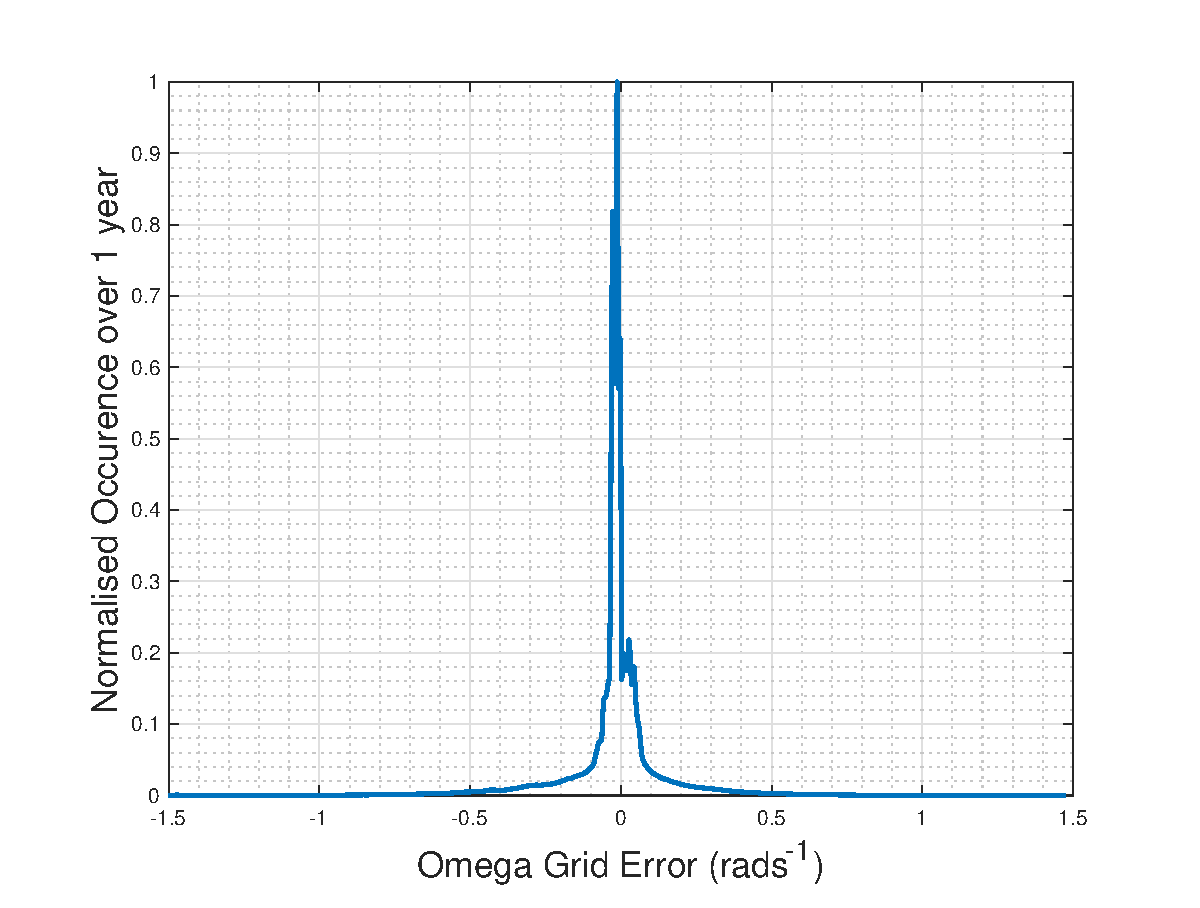
\includegraphics[width=1\linewidth]{images/results/omegafreq.eps}
  \caption{Simulation results showing the distribution of grid frequency errors.}
  \label{fig:omegaspread}
\end{subfigure}%
\begin{subfigure}{.5\textwidth}
  \centering
  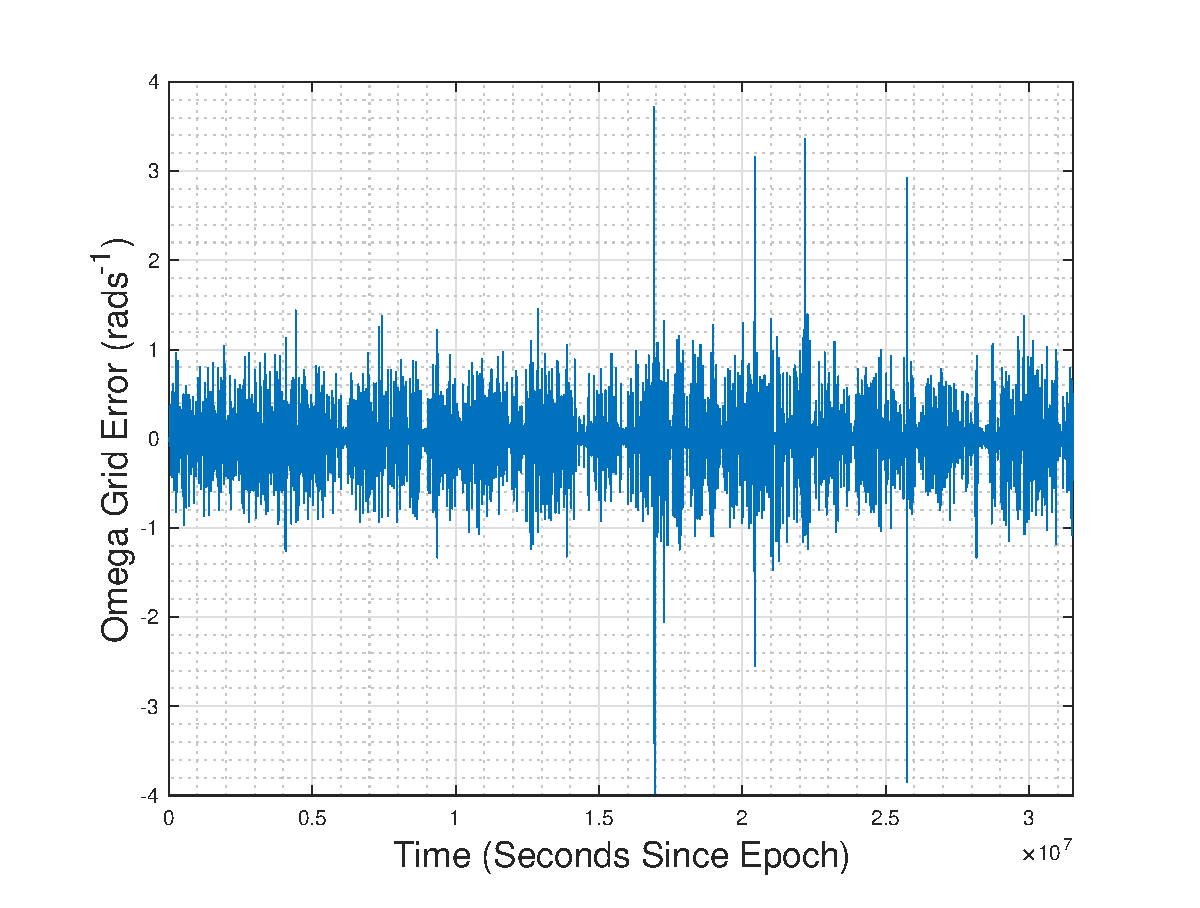
\includegraphics[width=1\linewidth]{images/results/omegayear.eps}
  \caption{Simulation results showing time series of grid frequency error.}
  \label{fig:omegayearseries}
\end{subfigure}
\caption{Simulation results from a 365 days of data, {\bf Augmented State LQR in parallel with LQR Applied.}}
\label{fig:omegastuff}
\end{figure}




%%%% YEAR SIM PART 5



\begin{figure}[ht]
\centering
\begin{subfigure}{.5\textwidth}
  \centering
  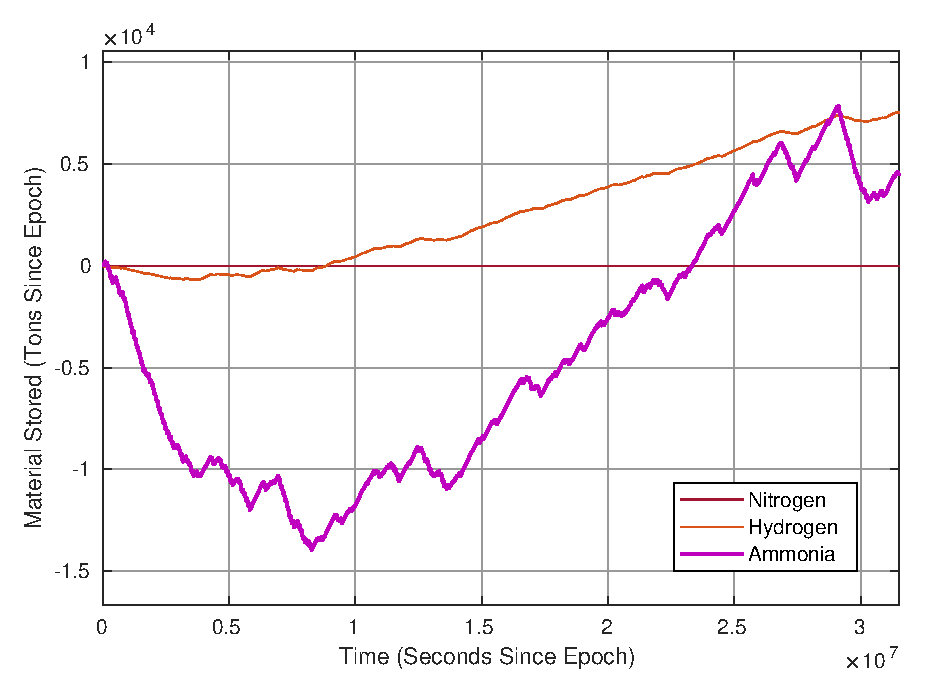
\includegraphics[width=1\linewidth]{images/results/tankyear.eps}
  \caption{Simulation results showing material balance for a year.}
  \label{fig:tankyear}
\end{subfigure}%
\begin{subfigure}{.5\textwidth}
  \centering
  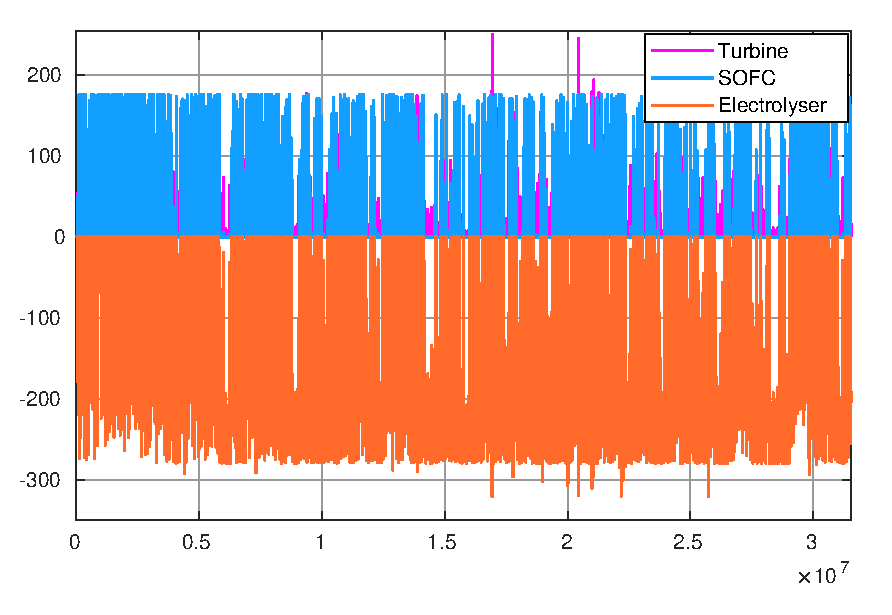
\includegraphics[width=1\linewidth]{images/results/useyear.eps}
  \caption{Simulation results showing component utilisation for a year.}
  \label{fig:useyear}
\end{subfigure}
\caption{Simulation results from a 365 days of data, {\bf Augmented State LQR in parallel with LQR Applied.}}
\label{fig:materialyear}
\end{figure}

To conclude this section, the Linear Quadratic Regulator was a good candidate for controlling the plant, which appears viable given the year's material balance from the simulations run.